%%\documentclass[12pt]{article}
\documentclass[12pt]{elsarticle}
\usepackage{graphicx}
\usepackage{subfig}
\usepackage{amssymb,hyperref,rotating}
%\usepackage{draftwatermark}
%\SetWatermarkScale{2.0}
%\usepackage{dcolumn}
%\usepackage{bm}
%\documentstyle{psfig,epsf}{article}
%\usepackage{psfig,wrapfig,floatfig,float}
%\topmargin 0.5cm
%\addtolength{\evensidemargin}{-1.5cm}
%\addtolength{\oddsidemargin}{-1.5cm}
%\addtolength{\textwidth}{2.54cm}
%\addtolength{\topmargin}{-1.5cm}
%\addtolength{\textheight}{2.54cm}

\topmargin=-0.25in
\textwidth=6.25in
\textheight=8.25in
%\textheight=9.25in
\oddsidemargin=0.125in
\evensidemargin=0.125in

%\addtolength{\textwidth}{1.2in}
%\addtolength{\topmargin}{-.7in}
%\addtolength{\leftmargin}{-1.1in}
%\addtolength{\footskip}{-1.5cm}
%%\setlength{\textheight}{9.25in}
%\setlength{\textheight}{9.3in}
%%\setlength{\parindent}{1em}
%\setlength{\parskip}{1ex}
%%\pagestyle{headings}
%\setlength{\oddsidemargin}{0.in}
%\setlength{\evensidemargin}{0.in}
%\renewcommand{\thepage}{Eric D. Church/page \arabic{page}}
\thispagestyle{empty}

\pagestyle{myheadings}
\begin{document}
\title{The Liquid Argon Offline Software Package: LArSoft} 
\author{Jonathan Asaadi}
\address{}
\ead{jaasaadi@syr.edu}
\author{Bruce Baller}
\address{}
\ead{baller@fnal.gov}
\author{Ben Carls}
\address{}
\ead{bcarls@fnal.gov}
\author{Eric Church}
\address{Fermi National Accelerator Lab, Batavia, IL, USA, 60510-5011}
\ead{echurch@fnal.gov}
\author{Bonnie Fleming}
\address{Physics Department, Yale University, New Haven, CT, USA, 12345-1234}
\ead{bonnie.fleming@yale.edu}
\author{Herb Greenlee}
\address{Fermi National Accelerator Lab, Batavia, IL, USA, 60510-5011}
\ead{greenlee@fnal.gov}
\author{Ben Jones}
\address{Massachusetts Institute of Technology, 77 Massachusetts Ave, Cambridge, MA 02139}
\ead{bjpjones@mit.edu}
\author{Wes Ketchum}
\address{}
\ead{wketchum@lanl.gov}
\author{Jim B. Kowalkowski}
\address{Fermi National Accelerator Lab, Batavia, IL, USA, 60510-5011}
\ead{jbk@fnal.gov}
\author{David McKee}
\address{}
\ead{mckee-d@mssu.edu}

\author{Gianluca Petrillo}
\address{Fermi National Accelerator Lab, Batavia, IL, USA, 60510-5011}
\ead{petrillo@fnal.gov}
\author{Brian Rebel}
\address{Fermi National Accelerator Lab, Batavia, IL, USA, 60510-5011}
\ead{brebel@fnal.gov}
\author{William Seligman}
\address{}
\ead{seligman@nevis.columbia.edu}
\author{Erica Snider}
\address{Fermi National Accelerator Lab, Batavia, IL, USA, 60510-5011}
\ead{rs@fnal.gov}
\author{Mitchell Paul Soderberg}
\address{Fermi National Accelerator Lab, Batavia, IL, USA, 60510-5011}
\ead{soderber@fnal.gov}

\author{Andrzej Szelc}
\address{}
\ead{andrzej.szelc@yale.edu}

\author{Kazuhiro Terao}
\address{}
\ead{kazuhiro@nevis.columbia.edu}
\author{Matthew Toups}
\address{}
\ead{mtoups@mit.edu}
\author{Tingjum Yang}
\address{Fermi National Accelerator Lab, Batavia, IL, USA, 60510-5011}
\ead{tjyang@fnal.gov}
%%\hspace{2cm}                         
\begin{abstract}
A common software package for the simulation, reconstruction, and analysis of Liquid Argon TPC (LArTPC) detectors is being developed as a collaboration across multiple experiments at Fermilab, with the core framework supported by Laboratory staff. We describe the architecture of the software and collaboration that provides the value delivered by the common package. We then describe the various components explaining the development and integration model for the common and experiment specific aspects – including the core framework, detector geometry, electronics response, package configuration, and algorithms. Finally we describe how LArSoft is being used, and in development for being used, by the multiple experiments that are participating.

\end{abstract}
\tableofcontents

%\large
%%%
%%%\clearpage
\maketitle

\section{Introduction}
\subsection{What is LArSoft}
LArSoft is a software package for the simulation, reconstruction, and analysis of all planned and running liquid argon experiments at Fermilab. Any Liquid Argon Time Projection Chamber (LArTPC) experiment can make use of LArSoft algorithms as long as the experiment supplies a properly formatted description of its detector geometry and electronics. 

LArSoft  benefits from the experience of multiple experiments.  Each LArTPC provides essentially the same basic information after accounting for small detector differences.  Thus, algorithms developed for one experiment can be directly used by another, as long as the differences in geometry are properly accounted for in the algorithms.  

A liquid argon detector and a sophisticated software toolkit can analyze event topologies typical of neutrino interactions that are difficult to parse and make sense of in traditional legacy technologies. Figure~(ADD bubble chamber and Liquid Argon results picture)
Liquid argon detectors see every nuance of the event. LArSoft applies reconstruction algorithms to identify clusters of energy deposit, tracks, particle showers, and iteration vertices.

\subsection{Who Uses LArSoft}
LArSoft is the product of the collaboration between the following experiments and Fermilab.
\begin{enumerate}
\item ArgoNeuT
\item LArIAT
\item MicroBooNE
\item LBNE
\item LAr1-ND
\end{enumerate}

\hspace*{2cm}
\begin{figure}[h]
\centering
%\caption{\subfloat[]{\includegraphics[width=3.0in]{picture of bubble chamber}}%
%\caption{\subfloat[]{\includegraphics[width=3.0in]{picture of liquid argon}}%
\label{bubble}
\end{figure}


\section{Framework and Tools}
\subsection{ART}
The foundation of LArSoft is the ART event processing framework which coordinates event processing via configurable, pluggable modules that add data to, and retrieve data from, events.\cite{art-ref}  An event is one unit of data. It may represent an interaction or any period of collected data.

ART provides many of the services necessary to operate in a production environment, include tools for compiling, installing, packaging, and deploying the system.  ART is developed and support by the Fermilab Scientific Computing Division (SCD) and is used by experiments within the neutrino, astrophysics, and muon programs, including NOvA, Muon G-2, Mu2e, and DarkSide-50, and alongside LArSoft for MicroBooNE, ArgoNeuT, and Lariat.

\subsection{External Packages}
\subsubsection{Event Generation}
LArSoft makes use of the NuSoft packages that provide a common interface to event generators, Geant4 and event display libraries developed for use by all neutrino experiments. The packages used include:    EventDisplayBase, EventGeneratorBase, G4Base, MagneticField, NuReweight and SimulationBase.

There are four different ways to create events for LArSoft:
\begin{enumerate}
\item{CRY - a third-party package to simulate cosmic rays documented at \cite{cry}}
\item{GENIE - external neutrino interaction generator used to produce neutrinos in the Monte Carlo simulation}
\item{Single - creation of single participle spill or multiple particles with the initial position, momenta, and the spread of momenta and starting positions specified in the job file.}
\item{LightSource - simulation of placing an extended, isotropic light source within the TPC volume to generate a stream of photons.}
\end{enumerate}

\subsubsection{Detector Simulation}
NEED WORDS

\subsection{Geometry Description Requirements}
LArSoft uses the Geometry Description Markup Language (GDML) which is an application-independent geometry description format based on Extensible Markup Language (XML.) 
The Geometry package contains a general interface into the detector descriptions of the different experiments so other packages do not depend on the detector. 

\begin{figure}[h]
\center
\caption{LArSoft requires a descending volume hierarchy of volWorld, volDetEnclosure, volCryostat, volTPC, volTPCPlane, volTPCWire to search for each of these specific volumes. There can be, and probably should be, multiple TPCPlanes and TPCWires.}
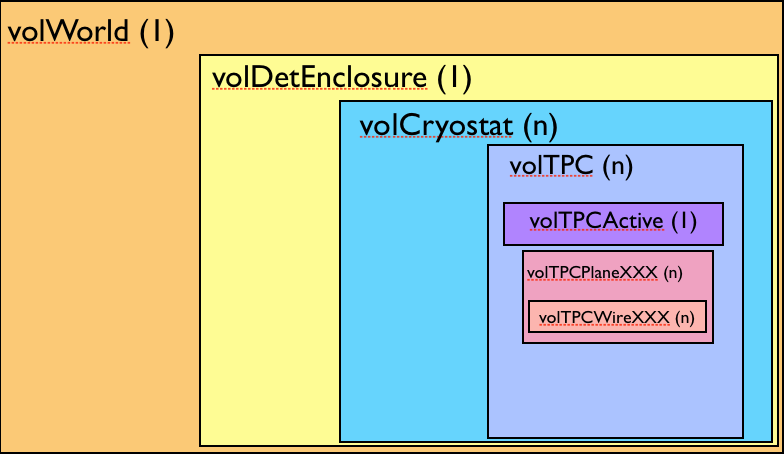
\includegraphics[width=4.0in]{./imgs/geometry_volumes.png}
\label{geo-vol.img}
\end{figure}

As shown in Figure~\ref{geo-vol.img},
the highest level volume is World which contains all elements of the geometry to be accounted for in the simulation and should be sized adequately to account for any features of the detector surroundings that are important for the simulation. For example, if there is a huge mass of rock near the detector that could alter the cosmic ray flux from that direction, it should be simulated. There is only one detector enclosure volume which can contain many Cryostat volumes, which in turn can each contain many TPC volumes. Each TPC volume contains only one TPCActive volume, which defines the active volume of liquid argon that is read out by the detector. Any liquid argon that is outside of the drift field would not be part of volTPCActive. It is assumed that volTPCActive is simply a volume of liquid argon with no sub-volumes in it. 

The TPC volume contains many TPCPlaneXXX volumes that describe the wire planes. The TPCPlaneXXX volume contains many TPCWireXXX volumes that each describe a wire in the detector. The Geant4 binding and the ROOT binding support the GDML import and export for reading GDML files and writing out GDML files.
                    
\section{Simulation Mechanics}

\subsection{Data Product Description}
LArSoft simulation jobs are modular in nature, with each module reading input data objects and writing output data objects to the event.  
As the readout electronics differ for each experiment using LArSoft, each
experiment must provide a detailed simulation of its electronics. 
\subsection{Adaptations for Using G4}
- LArSoft specific adaptations for using G4 (the user action lists and readout geometries)
The truth particles generated in the event generator step are passed to a Geant4 based detector simulation called LArG4.  The geometry GDML file is parsed to create a Geant4 detector description using the built-in GDML parser, which interfaces to LArSoft via the DetectorConstruction LArSoft class.
\subsubsection{User Action Lists}
NEED WORDS.
\subsubsection{Readout Geometries}
NEED WORDS
\subsection{Adding Additional Detectors}
- hooks for adding in additional detectors outside of the LAr volumes. 
NEED WORDS.
\subsection{New Parameterizations for Ionization}
- description of how new parameterizations for ionization, etc can be added into the simulation including a description of the mechanism for calculating the amount of ionization charge and scintillation light.  It could include a statement of the available options for that calculation (NEST vs decoupled charge and light) and how a user might add a new method.
NEED WORDS

\subsection{Incorporating Magnetic Fields}
LArSoft provides limited support for simulating magnetic
fields. A constant and uniform field may be specified
throughout any single volume (and it's sub-volumes) of the Geant
geometry, and will be respected by Geant's particle tracking
algorithms. There is currently no support for altered electron
drift directions, nor any explicit support for analyzing events
in the presence of a non-zero magnetic field.\footnote{Both of these features are planned.}

\subsection{Optical Simulation}
Optical physics simulations in LArSoft can take one of two forms: full or fast simulation.  Both optical simulations are implemented within LArSoft's GEANT4 based simulation package and make use of its configurable physics list functionality.  This functionality allows LArSoft simulations to define a custom GEANT4 physics list from a set of physics constructors at runtime, and is used to select between full optical, fast optical or no optical simulation. 

\subsubsection{Full Optical Simulation}
The full simulation involves stepping individual photons through the detector volume.  Each stepping photon is treated as an individual particle in Geant4.  The number of photons stepped is usually reduced by a constant factor representing the optical detector collection efficiency at 128 nm, thereby scaling the photon count at production rather than detection in order to reduce computation time and memory usage. 

The physics constructor for full optical physics in LArSoft has been adapted from the standard GEANT4 optical physics constructor. Default implementations for scintillation and Cerenkov production, Rayleigh scattering and absorption at boundaries and in the bulk are included. The default implementation of wavelength shifting physics processes is also included, although at present most LArSoft experiments incorporate the wavelength shifting physics into an estimate of the optical detector collection efficiency rather than simulating it at the photon-by-photon level.  A customized, faster reflectivity model is implemented, whereby material boundaries have specified diffuse and specular reflectances which for each material boundary type.  

Properties of the liquid argon volume including its optical characteristics are loaded into LArSoft by a dedicated service and as such are globally accessible within the LArSoft framework.  This allows reconstruction as well as simulation algorithms to access important optical properties.  The full optical physics processes within LArSoft are configured as follows:

Scintillation production is configured with a photon momentum spectrum centered at 9.7 eV and a shape which is taken from \cite{spectrum}.  Singlet and triplet scintillation components are included, with time constants of 6 and 1500 ns, although tensions within the literature suggests these will require finer tuning using data from LArSoft experiments \cite{fastslow}.  The scintillation yield can is defined per incident particle type using an extension of the relationship shown in \cite{scintyield}, and the absolute yield for a minimum ionizing particle is set to 24,000 photons per MeV, assuming a constant electric field strength of 500 V / cm. 

Cerenkov photons are produced with yields and energies corresponding to the standard Frank-Tamm spectrum of Cerenkov radiation, given a continuous parameterization of the liquid argon refractive index derived from the references in \cite{RIndex}. Rayleigh scattering and photon-absorption process are enabled, where the scattering length is specified over the range of photon energies from 1.8 eV to 10.8 eV, and is 90 cm at the peak of the argon scintillation spectrum \cite{Rlength}.  The bulk absorption length is set to 2000 m (approximately infinite). Further work to parameterize purity dependent absorption effects may be required, with absorption due to dissolved nitrogen being the most likely additional effect \cite{nitrogen}.

A simplified reflectivity model is used, whereby each type of boundary in the detector is supplied with a wavelength dependent total reflectivity and specular/diffuse reflection fraction.   For  preliminary  studies  only the  steel/argon boundaries  at  the  edge of the cryostat are  reflective,  with  all  other  surfaces,  including  wires,  field cage,  etc,  being opaque.   The steel/argon boundaries have a total reflectance of 25\%, of which 50\% is specular, with these numbers being taken from \cite{reflectances}.  

\begin{figure}[t]
\centering
\caption{Illustration of the simple treatment of wireplane absorption in LArSoft}
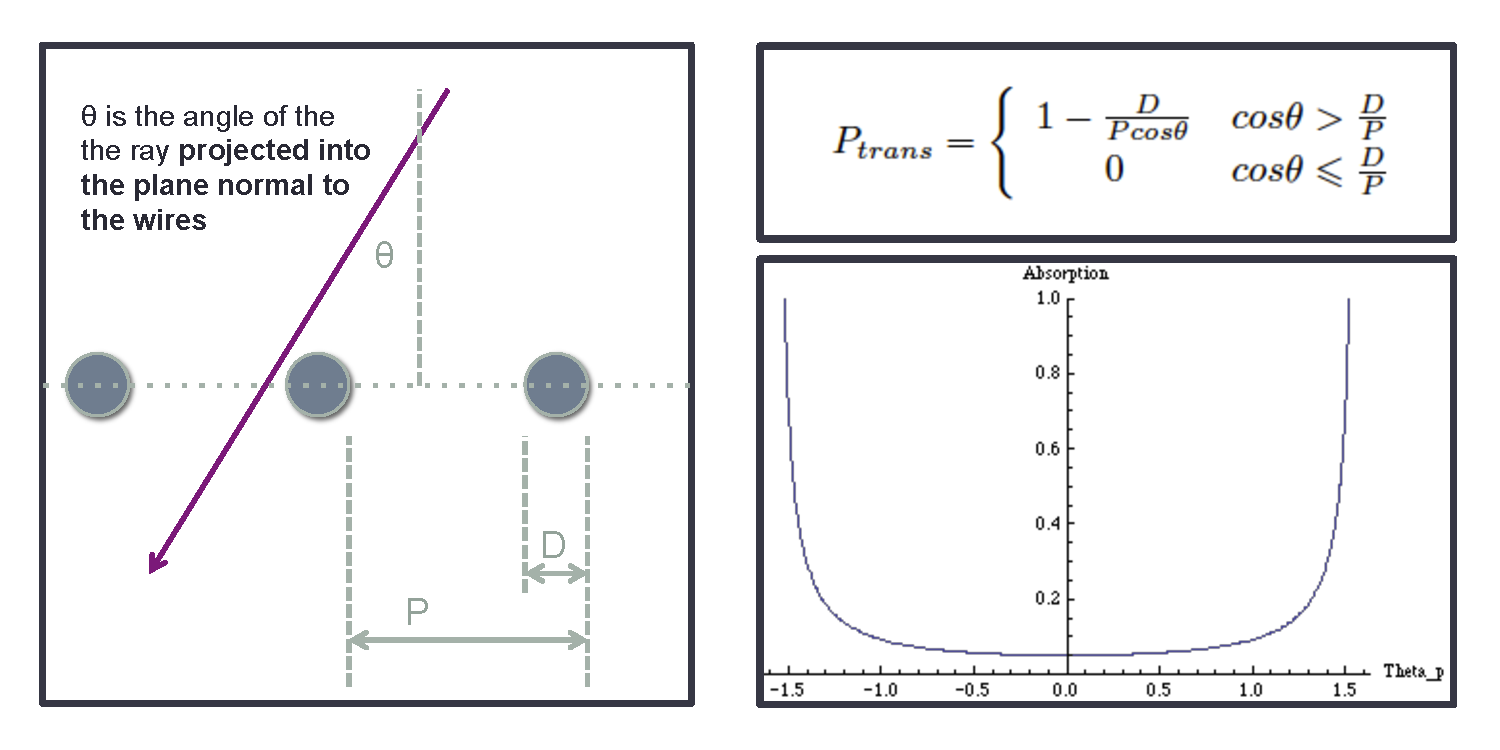
\includegraphics[width=6.0in]{./imgs/WireplaneTransmissionCartoon.pdf}
\label{fig:wireplaneabs}
\end{figure}


Semi-transparent surfaces are also included.  For a given surface, any angularly dependent transmission spectrum can be incorporated.  This allows a modeling of the non-uniform angular dependence of photon transmission through the detector wireplanes.    LArSoft includes derived classes which implement optical attenuation by one or many planes of cylindrical wires which are assumed black to 128 nm light.  A cartoon of the wireplane opacity model is shown in figure \ref{fig:wireplaneabs}.

Photons are counted at detector volumes whose name matches a string supplied to the LArSoft geometry service.  This volume may represent a photomultiplier tube, or else another element defined as optically sensitive, for example, a wavelength shifting surface. At geometry construction time, the volumes matching the appropriate name string in the gdml file are assigned optical detector IDs and become sensitive within the LArSoft simulation.

The sensitive elements are placed in a separate GEANT4 parallel world geometry (one of three used in LArSoft - see figure \ref{fig:parallelgeom}).  Only photons are tracked in this geometry, which ensures that the optical  detection process is triggered only for optical photons.  This scheme also means that photon step size is not limitted by the TPC voxel size, which provides a significant performance improvement. Upon photon detection, tracking of the photon is stopped and information about its arrival time and detection location are stored in a detected photon table.  At the end of the run, this table is queried to generate simulated photon data products to store in the event.  The same table is filled by the fast simulation method, and hybrid fast and full simulations can be run.  One use case for such a hybrid simulation would be the fast simulation of scintillation photons but full simulation for Cerenkov photons, which have a directionality and so cannot be consistently treated by the fast simulation.


\begin{figure}[t]
\centering
\caption{A cartoon which illustrates the three parallel simulation geometries used in the LArSoft
GEANT4 implementation.}
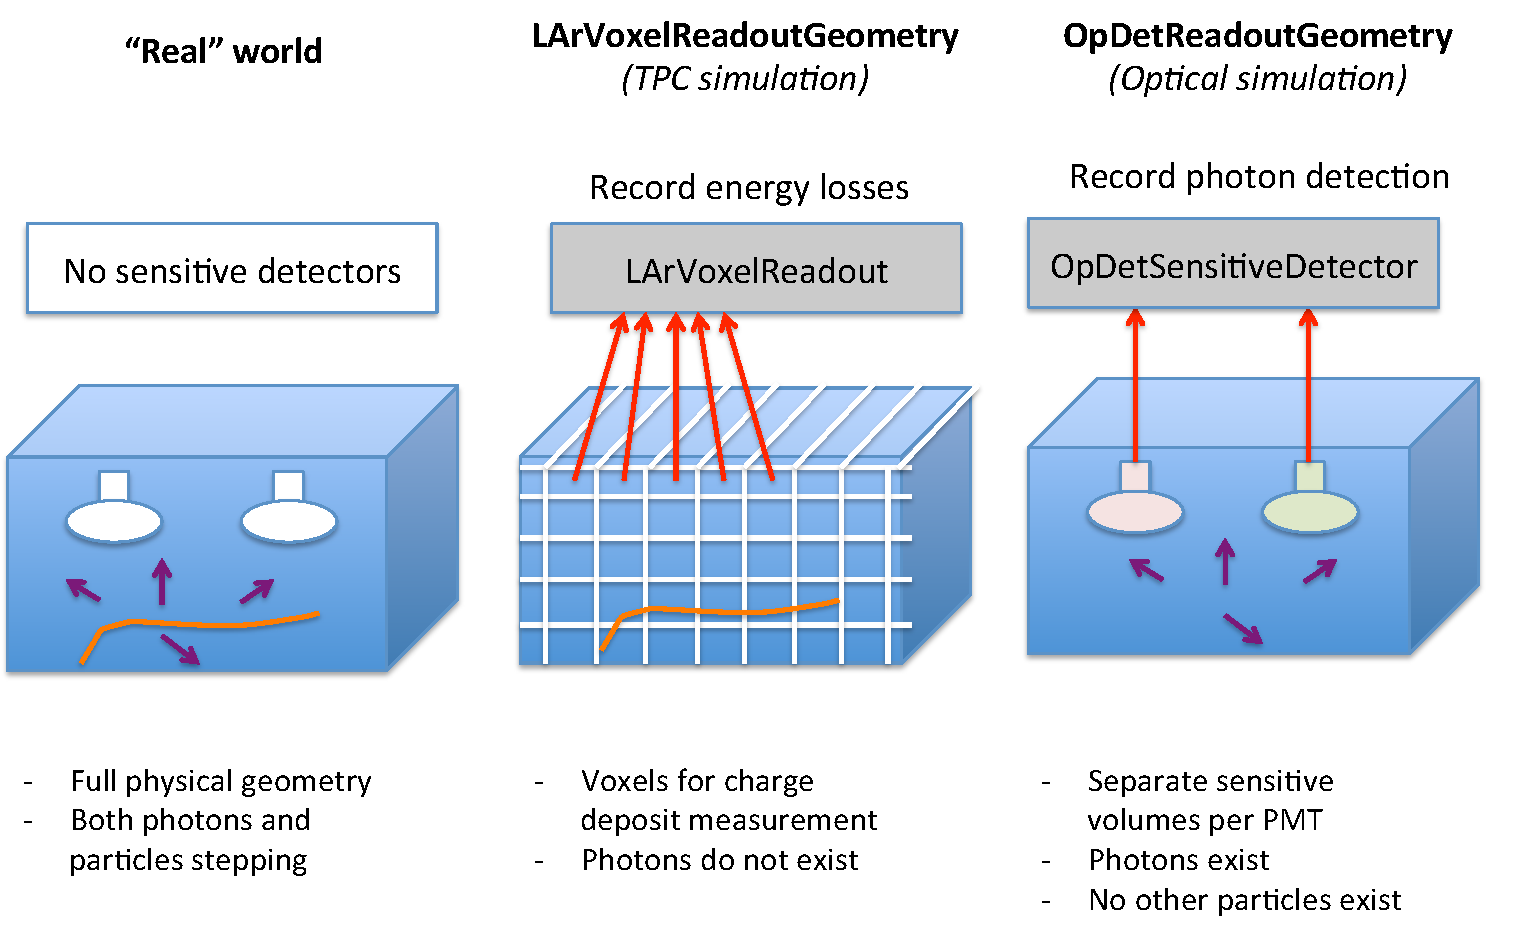
\includegraphics[width=6.0in]{./imgs/ParallelGeomScheme.pdf}
\label{fig:parallelgeom}
\end{figure}

\subsubsection{Fast Optical Simulation Modules}

Since the number of optical photons generated per event is of order tens of millions per GeV, full optical simulation is a very computationally intensive process.  Since scintillation in argon is isotropic, the visibility (defined as the fraction of generated photons which will reach a given optical detector) can be pre-calculated at each point in the detector.  The fast optical simulation takes this approach, to avoid stepping individual photons during routine simulation jobs.

The liquid argon volume of the detector is coarse-grained into optical voxels, the size of which must be chosen to be smaller than the resolution of the optical system but can be significantly larger than the TPC voxelization scale.  The optical fiducial volume incorporates the all detector volumes which are visible to the optical system, which in general extends further than the TPC fiducial volume.  By default, the complete cryostat volume is optically voxelized, although if there are invisible regions for a specific detector then a smaller optically active volume can be specified.

A dedicated run of the full optical simulation can be made to create a lookup table which contains the visibility of each voxel to each optical detector.  This run creates a specified number of isotropic 128 nm photons, uniformly distributed across each voxel volume at time t=0.  These photons propagate and are detected using the same mechanics as the full photon simulation.  After photon propagation, the number detected photons at each optical detector is used to build the optical visibility lookup table.  This process is automated by a dedicated photon visibility service, which communicates with the event generation, simulation and analysis parts of the simulation chain to ensure they are correctly configured when a look table building job is run.

Once the visibility table has been generated, the probability that a given 128 nm photon will reach a specified optical detector can be quickly accessed using the photon visibility service which is available to both simulation and reconstruction modules.  The LArSoft GEANT4 simulation can be configured to include the fast optical physics constructor which implements the lookup-based fast scintillation process within simulations. The generation parameters for scintillation light in the fast scintillation process are equivalent to those used in the full simulation.  However, instead of placing optical photons onto the GEANT4 particle stack, detected optical photons are inserted directly into the detected photon table probabilistically, based on the visibility of the detector location where the scintillation occurred.  The arrival times of the photons are also smeared based on the distribution of production times.  The sum of detected photons from each voxel where scintillation emission occured gives the total optical detector response.

The photon library is both geometry and voxelization scheme specific, and changes to either require a full regeneration, which is a one-time computationally intensive job.  The effects of rayleigh scattering and absorption are also built into the visibility table.  Changes to the argon scintillation production properties and optical detector efficiencies, on the other hand, can be made without regenerating the table.

\begin{figure}[t]
\centering
\caption{An example of slices through an optical visibility table. This shows the visibility at various points
in the MicroBooNE detector.  This plot was made from the optical visibility table using the optical library
analyzer module.}
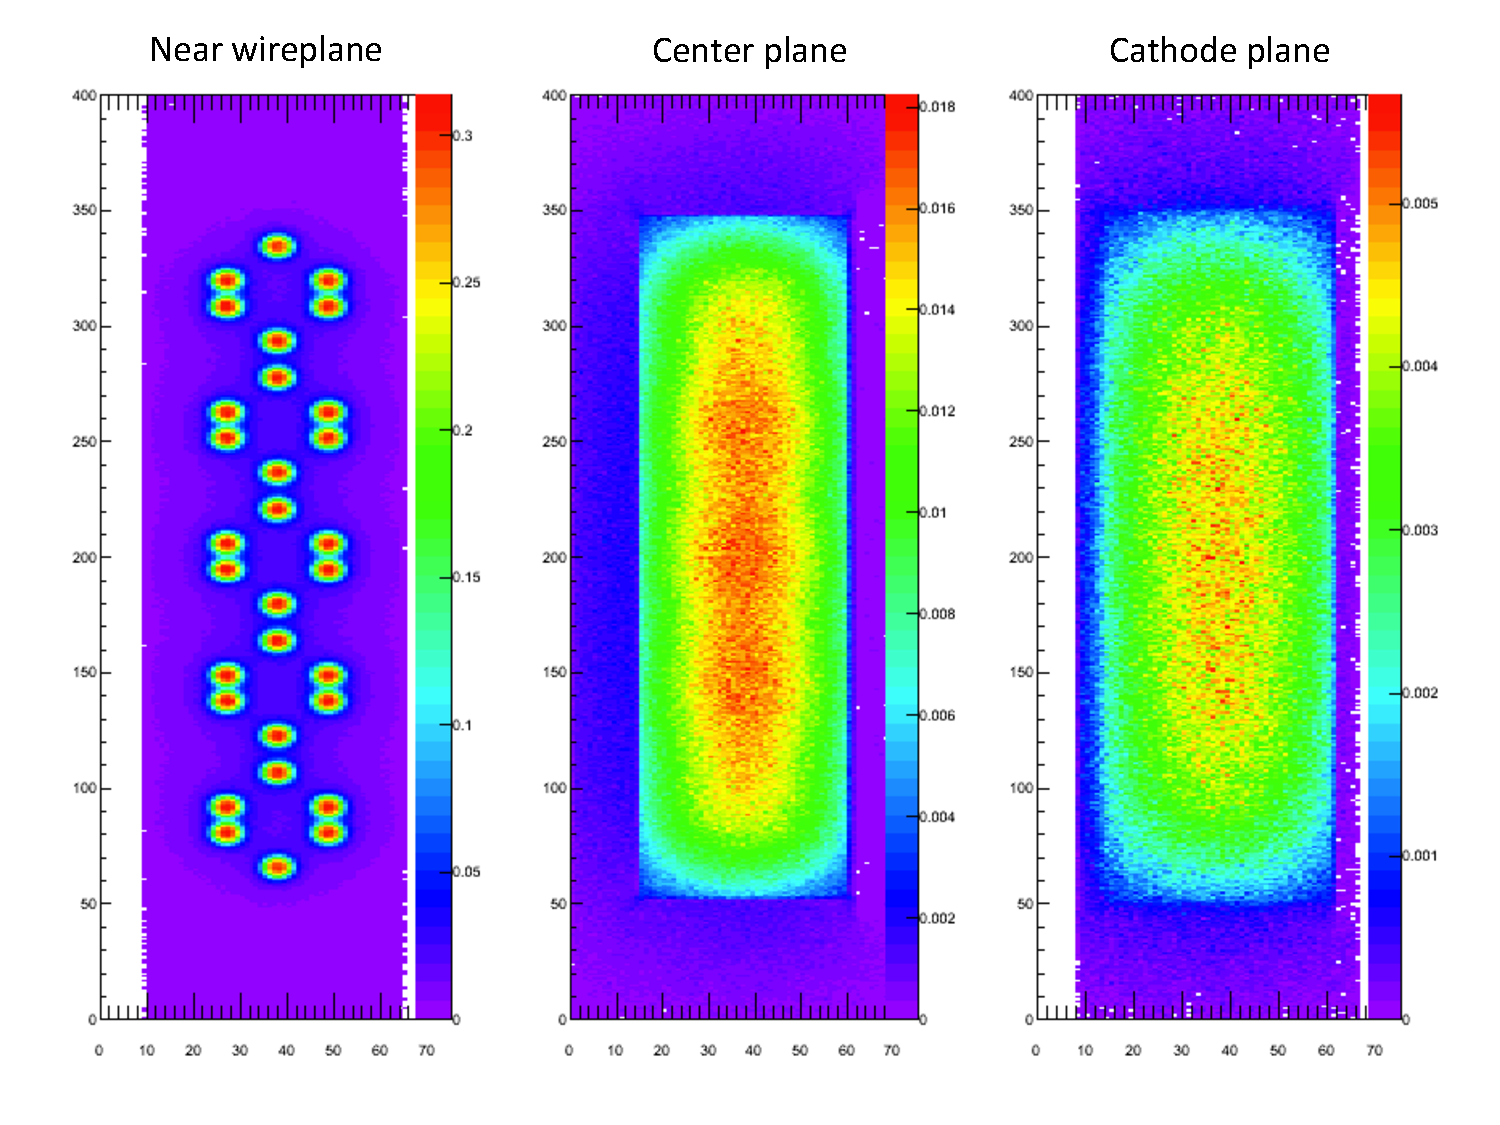
\includegraphics[width=6.0in]{./imgs/SampleOpticalMap.pdf}
\label{fig:opticalmap}
\end{figure}

\subsubsection{Tools for Optical Simulations}

There are several tools in LArSoft which are can be used for optical simulation validation and basic analysis.  The photon counter module is an analyzer which produces analysis trees and histograms representing the properties of the detected photons in each optical detector.  The module extracts per-optical-detector and per-event information and can be used for both full and fast simulation outputs.  This same module is also used to generate the optical visibility library used by the LArSoft fast simulation.

There is a light source event generator which can be configured to generate photons at a specified wavelength and with a specified geometry and time.  Optionally the light source can be configured to step through each optical voxel event-by-event, or else step through a custom set of arbitrary geometrical configurations specified in a text file.  This event generator is particularly useful for investigating the optical response to different event geometries and is used in the generation of the photon visibility library.

A library analyzer module exists to produce detector visibility maps and other histograms based on the loaded visibility library.  This module is used to validate the optical library and obtain information about the detector response to light deposits at different points.  Some histograms produced by this module for the MicroBooNE optical library are shown in figure \ref{fig:opticalmap}.



\section{Reconstruction Mechanics}
\subsection{Data Product Description}
The reconstruction chain proceeds in the following steps
\begin{enumerate}
\item First, the raw energy depositions (digits) are calibrated into signals on wires.
\item Next, hits are formed from the regions containing wire signals that are above a tunable threshold.
\item Hits are then grouped into clusters.
\item Clusters are classified to be projections from either 3D tracks or showers. Tracks and showers inherit from the class prong, in the usual C++ sense.
\item Vertices are located using prongs that are shown to originate from a common point.
\item Finally, prongs and vertices are associated into events.
\end{enumerate}
The LArSoft reconstruction chain is complete in that initial algorithms for each step currently exist.  More effort will be required to demonstrate that every, or at least most of the desired, event topologies can be handled in an automated way in the reconstruction chain. Detailed studies of various event classes are in progress to understand the performance of each reconstruction algorithm.

The reconstruction algorithms in LArSoft have benefited from several advances in image analysis techniques developed over the past decade.  For example, the algorithm used to cluster groups of energy depositions together is directly taken from the heavily-cited work of Ester, Kriegel, Sander, and Xu's~\cite{ester} Density Based Spatial Clustering of Applications with Noise (DBSCAN). The two-dimensional (2D) vertex, or more accurately line-endpoint, finding algorithms are based on a corner finding technique used for locating edges and corners in photographic images.  Initial particle tracking is performed using Hough line finding techniques.

\hspace*{2cm}
\begin{figure}[h]
\centering
\caption{This flow chart shows the objects created along a possible reconstruction chain in LArSoft.}
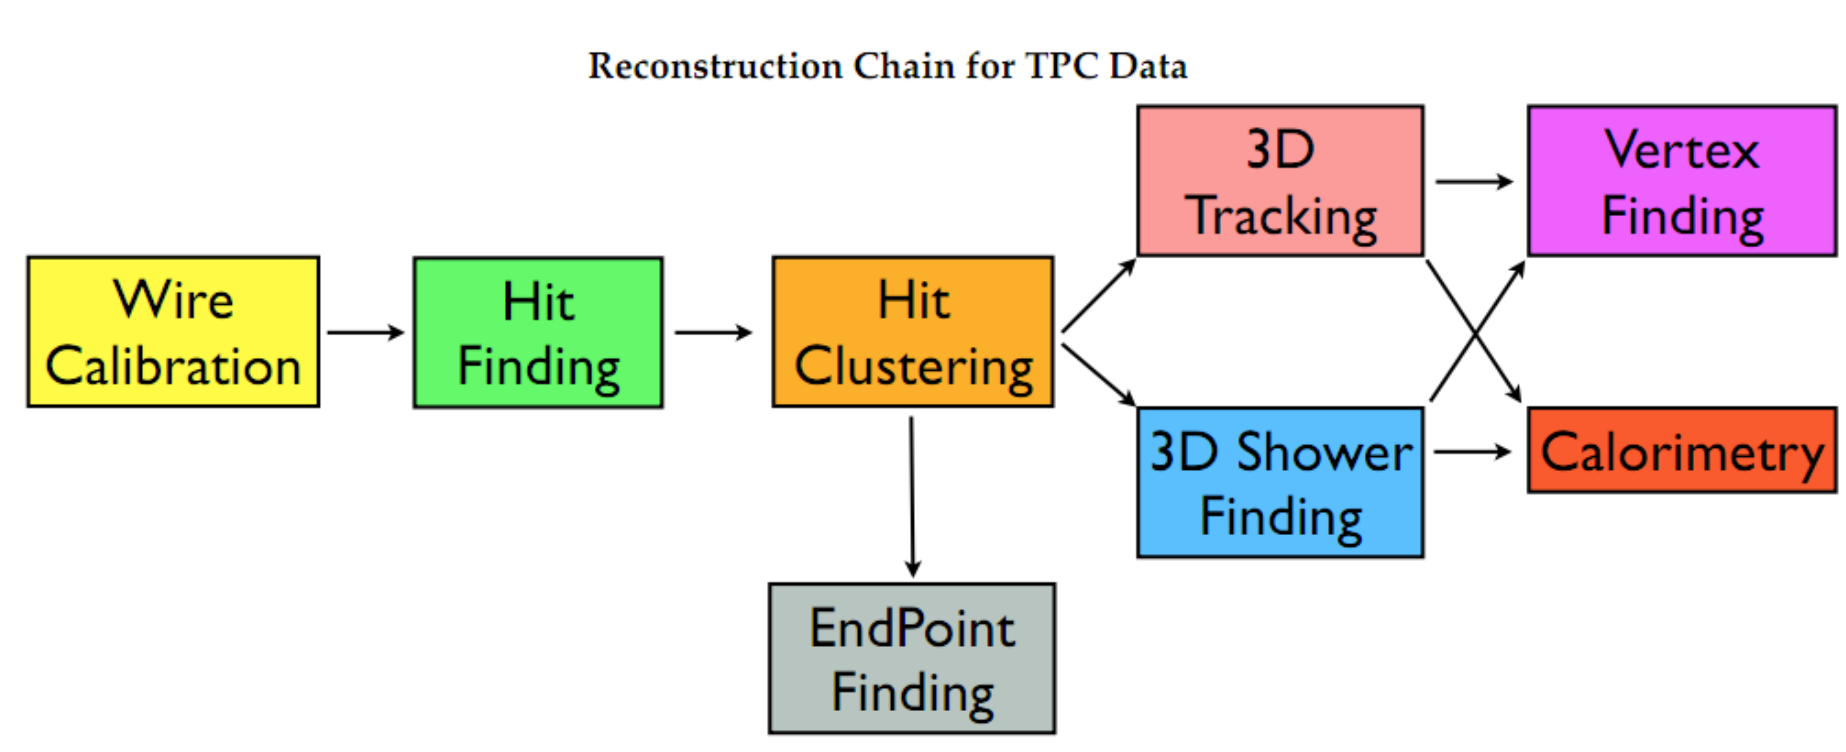
\includegraphics[width=4.0in]{./imgs/LArSoft-Recon-Flow-Soderberg.png}
\label{flow}
\end{figure}

ADD picture -- Another reconstruction chain in LArSoft

Reconstruction in LArSoft has both 2D and 3D portions. The reconstruction does not have to proceed by building 2D information before creating 3D information, but the option to do so exists. 

\subsection{Organization of Algorithms}

What is an algorithm? How do they relate to modules?

\subsection{Implementation Plan for Algorithms and Modules}
NEED WORDS.

\subsection{Unique aspects of LArSoft Reconstruction}

\subsection{Event Visualization}
LArSoft has an event display.
It can be used for
\begin{enumerate}
\item{MC}
\item{Data}
\item{2D}
\item{3D}
\end{enumerate}  

Figure~\ref{argo.evd} shows an example event display for an ArgoNeuT data event.

\hspace*{2cm}
\begin{figure}[h]
\centering
\caption{A data event in ArgoNeuT, viewed with the event display in LArSoft. Among other emitted particles, two $\pi^0$s are evident.}
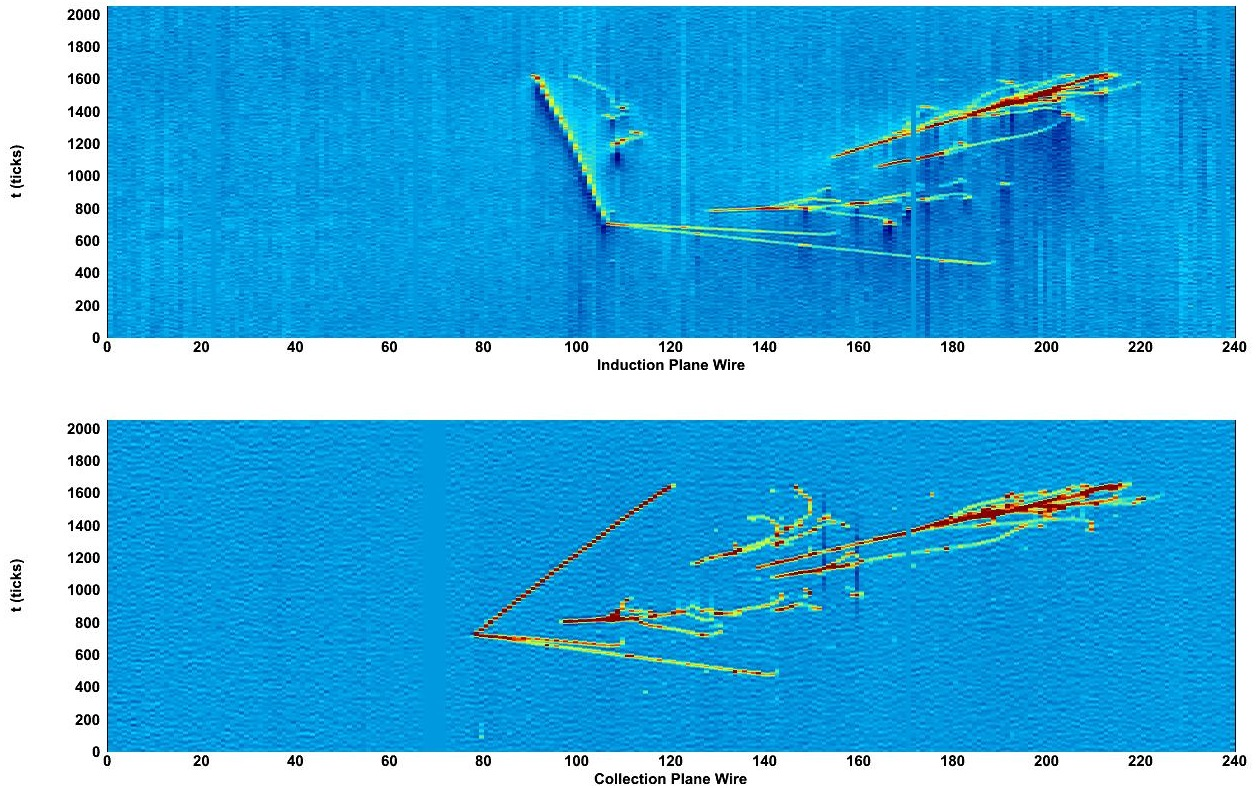
\includegraphics[width=4.0in]{./imgs/ArgoNeuT_event.jpg}
\label{argo.evd}
\end{figure}



               
\section{Analysis Mechanics}

\subsection{Data Product Description}
NEED WORDS.

\subsection{Organization of Algorithms for Analysis}
NEED WORDS.

\subsection{Implementation Plan}
NEED WORDS.

\subsection{Unique Analysis Aspects of LArSoft}
NEED WORDS.

\section{Getting Software and Benchmarking it}
\subsection{Ways to Contribute}

LArSoft general software is hosted in ten GIT repositories with additional experiment-specific repositories for digitization code and configuration files. MultiRepository Build (MRB) compiles code across GIT repositories. Each repository has a test area and some libraries such as EventGenerator, LArG4, HitFinder, VertexFinder, etc.\cite{gian}

To avoid having one developer's code negatively impact other software and to allow for vetting before others use the new software, no development takes place directly on the develop branch of the repository. LArSoft uses the git-flow\cite{git-flow} model which makes it easy for users to have a private version of the software they are working on. Nothing gets included in the develop branch until the changes are tested.\cite{git-control} All LArSoft developers are expected to follow this workflow model in order to maintain the integrity of the develop branch.

A group of people, the librarians, vet the code going into all releases. The librarians examine the changes made to the software in detail as well as looking at the bigger picture to ensure the software module performs the expected task(s). In particular, they ensure that the new code does not negatively impact other LArSoft software. Librarians also ensure the new code is documented and that tests are provided.

Librarians interact with the authors until the code meets the tenants listed at \cite{code-tenants}. LArSoft code is intended to be usable by Liquid Argon TPC with any number of planes, wires, or PMTs. In addition, the code should be flexible and well-documented. 

\subsection{Testing}

In LArSoft, there is unit testing and integration testing which includes regression tests. The integration tests are written by the author, but may be tested by other people in the project as well as the author. It must be possible to run integration tests automatically as well.

LArSoft has set up a Continuous Integration system based on Jenkins\cite{jenkins} that routinely performs a sequence of tests including unit tests, integration tests and regression tests. On failure, the automatic system notifies LArSoft personnel who contact the responsible person(s) to fix the error.

\subsection{Resource Usage}

A rough estimate of resource usage can be optained by running standard ART services called TimeService and SimpleMemoryCheck. TimeService gives an estimate of the time used by the module to perform its task. SimpleMemoryCheck monitors the usage of memory (RAM) by the whole program. In order for jobs to run smoothly in a GRID or remote environment, the job should use less than 2 Gigabyte of memory, and less than 48 hours (Gianluca will check) of CPU time.

A resource coordinator in LArSoft cheeks for excessive usage, and if found, analysis is done using tools like Valgrind\cite{valgrind}, Gperftools\cite{gperf}, and Allinea.\cite {allinea}.
The code author is notified by the resource coordinator of the issue and they develop a solution to the resource problem. Most typical problems relate to the use of data structures, and can be solved by following the ART guidelines.\cite{art-guide}
 
\section{Summary}
NEED WORDS.
\section{References}

\begin{thebibliography}{99}
\bibitem{wcsim} https://wiki.bnl.gov/dusel/index.php/Simulation/Software
\bibitem{ester} Ester, M., Kriegel, H.-P., Sander, J., and Xu, X. 1996. "A density-based algorithm for discovering clusters in large spatial databases with noise," Proc. 2nd Int. Conf.
\bibitem{art-ref} https://cdcvs.fnal.gov/redmine/projects/artdaq
\bibitem{cry} http://nuclear.llnl.gov/simulation/
\bibitem{gian} Petrillo, Gianluca, 2014. "LArSoft: simulation and reconstruction for Liquid Argon TPC," Liquid Argon TPC R\&D Workshop, Fermilab.
\bibitem{git-flow} https://cdcvs.fnal.gov/redmine/projects/cet-is-public/wiki/Git\_flow\_quick\_start
\bibitem{git-control} https://cdcvs.fnal.gov/redmine/projects/larsoft/wiki/\_The\_developer\_environment\_
\bibitem{code-tenants} https://cdcvs.fnal.gov/redmine/projects/larsoft/wiki/The\_rules\_and\_guidelines
\bibitem{jenkins} http://jenkins-ci.org/
\bibitem{valgrind} http://valgrind.org/
\bibitem{gperf} https://code.google.com/p/gperftools/
\bibitem{allinea} http://www.allinea.com/
\bibitem{nest} http://nest.physics.ucdavis.edu/site/
\bibitem{spectrum} E. Morikawa et al. "Argon, krypton, and xenon excimer luminescence: From the dilute gas to the condensed phase." J. Chem. Phys, 91:1469, 1989.
\bibitem{scintyield} Tadayoshi Doke, Akira Hitachi, Jun Kikuchi, Kimiaki Masuda, Hiroyuki Okada, and Eido Shibamura. "Absolute scintillation yields in liquid argon and xenon for various particles." Japanese Journal of Applied Physics, 41(Part 1, No. 3A):1538–1545, 2002.
\bibitem{fastslow} A Hitachi et al. "Effect of ionization density on the time dependence of luminescence from liquid argon and xenon", Phys. Rev. B 27:5279 (1983). P. Cennini et al, "Detection of scintillation light in coincidence with ionizing tracks in a liquid argon time projection chamber." NIM A: 432(23):240–248, 1999.  R. Acciarri et al, Effects of Nitrogen contamination in liquid Argon, 2008 JINST 5 (2010) P06003.  D. Whittington and S. Mufson, "Scintillation Light from Cosmic-Ray Muons in Liquid Argon", 2014, arXiv:1408.1763
\bibitem{reflectances} M Antonello et al.  "Analysis of Liquid Argon Scintillation Light Signals with the ICARUS T600 Detector".  Unpublished.
\bibitem{nitrogen} B.J.P. Jones et al, "A Measurement of the Absorption of Liquid Argon Scintillation Light by Dissolved Nitrogen at the Part-Per-Million Level", JINST 8 (2013) P07011
\bibitem{RIndex} A. C. Sinnock and B. L. Smith. "Refractive indices of the condensed inert gases." Phys. Rev. 181:1297–1307, May 1969.   R. K. Teague and C. J. Pings. "Refractive index and the lorentz–lorenz function for gaseous and liquid argon, including a study of the coexistence curve near the critical state." J Chem Phys, 48(11):4973–4984, 1968.
\bibitem{Rlength} G.M. Seidel, R.E. Lanou, and W. Yao, "Rayleigh scattering in rare-gas liquids", NIM A489 (2002) 189.   N. Ishida et al., "Attenuation length measurements of scintillation light in liquid rare gases and their mixtures using an improved reflection suppresser", NIM A384 (1997) 380. M. Sneep and W. Ubachs, "Direct measurement of the Rayleigh scattering cross section in various gasses", J. Quant. Spectrosc. Radiat. Transf. 92 (2005) 293.
\bibitem{art-guide} https://cdcvs.fnal.gov/redmine/projects/art/wiki/Guide\_to\_writing\_and\_using\_services
\end{thebibliography}
\clearpage 

\end{document}







